%%%%%%%%%%%%%%%%%%%%%%%%%%%%%%%%%%%%%%%%%
% University Assignment Title Page 
% LaTeX Template
% Version 1.0 (27/12/12)
%
% This template has been downloaded from:
% http://www.LaTeXTemplates.com
%
% Original author:
% WikiBooks (http://en.wikibooks.org/wiki/LaTeX/Title_Creation)
%
% License:
% CC BY-NC-SA 3.0 (http://creativecommons.org/licenses/by-nc-sa/3.0/)
%%%%%%%%%%%%%%%%%%%%%%%%%%%%%%%%%%%%%%%%%


%----------------------------------------------------------------------------------------
%	PACKAGES AND OTHER DOCUMENT CONFIGURATIONS
%----------------------------------------------------------------------------------------

\documentclass[10pp]{article}
\usepackage{geometry}
 \geometry{
 a4paper,
 total={170mm,245mm},%252
 left=20mm,
 top=25mm,
 }
\usepackage[english]{babel}
\usepackage[utf8x]{inputenc}
\usepackage{amsmath}
\usepackage{graphicx}
\usepackage[colorinlistoftodos]{todonotes}
% Copyright 2017 Sergei Tikhomirov, MIT License
% https://github.com/s-tikhomirov/solidity-latex-highlighting/

\usepackage{listings, xcolor}

\definecolor{verylightgray}{rgb}{.97,.97,.97}

\lstdefinelanguage{Solidity}{
	keywords=[1]{anonymous, assembly, assert, balance, break, call, callcode, case, catch, class, constant, continue, contract, debugger, default, delegatecall, delete, do, else, event, export, external, false, finally, for, function, gas, if, implements, import, in, indexed, instanceof, interface, internal, is, length, library, log0, log1, log2, log3, log4, memory, modifier, new, payable, pragma, private, protected, public, pure, push, require, return, returns, revert, selfdestruct, send, storage, struct, suicide, super, switch, then, this, throw, transfer, true, try, typeof, using, value, view, while, with, addmod, ecrecover, keccak256, mulmod, ripemd160, sha256, sha3}, % generic keywords including crypto operations
	keywordstyle=[1]\color{blue}\bfseries,
	keywords=[2]{address, bool, byte, bytes, bytes1, bytes2, bytes3, bytes4, bytes5, bytes6, bytes7, bytes8, bytes9, bytes10, bytes11, bytes12, bytes13, bytes14, bytes15, bytes16, bytes17, bytes18, bytes19, bytes20, bytes21, bytes22, bytes23, bytes24, bytes25, bytes26, bytes27, bytes28, bytes29, bytes30, bytes31, bytes32, enum, int, int8, int16, int24, int32, int40, int48, int56, int64, int72, int80, int88, int96, int104, int112, int120, int128, int136, int144, int152, int160, int168, int176, int184, int192, int200, int208, int216, int224, int232, int240, int248, int256, mapping, string, uint, uint8, uint16, uint24, uint32, uint40, uint48, uint56, uint64, uint72, uint80, uint88, uint96, uint104, uint112, uint120, uint128, uint136, uint144, uint152, uint160, uint168, uint176, uint184, uint192, uint200, uint208, uint216, uint224, uint232, uint240, uint248, uint256, var, void, ether, finney, szabo, wei, days, hours, minutes, seconds, weeks, years},	% types; money and time units
	keywordstyle=[2]\color{teal}\bfseries,
	keywords=[3]{block, blockhash, coinbase, difficulty, gaslimit, number, timestamp, msg, data, gas, sender, sig, value, now, tx, gasprice, origin},	% environment variables
	keywordstyle=[3]\color{violet}\bfseries,
	identifierstyle=\color{black},
	sensitive=false,
	comment=[l]{//},
	morecomment=[s]{/*}{*/},
	commentstyle=\color{gray}\ttfamily,
	stringstyle=\color{red}\ttfamily,
	morestring=[b]',
	morestring=[b]"
}

\lstset{
	language=Solidity,
	backgroundcolor=\color{verylightgray},
	extendedchars=true,
	basicstyle=\footnotesize\ttfamily,
	showstringspaces=false,
	showspaces=false,
	numbers=left,
	numberstyle=\footnotesize,
	numbersep=9pt,
	tabsize=2,
	breaklines=true,
	showtabs=false,
	captionpos=b
}

\usepackage{hyperref}
\usepackage{setspace}
\hypersetup{%
	pdfpagelabels=true,%
	plainpages=false,%
	pdfauthor={Dominic Hagmann, Jannik Brun, Lucien Erdin, Michael Vogel, Michel Perez, Thomas Keller, Toni Tanner},%
	pdftitle={Project-LESS},%
	pdfsubject={ETH Zurich, BIOTS2018},%
	bookmarksnumbered=true,%
	colorlinks=false,%
	citecolor=black,%
	filecolor=black,%
	linkcolor=black,%
	urlcolor=black,%
	pdfstartview=FitH%
}
\usepackage{fancyhdr}
 
\pagestyle{fancy}
\fancyhf{}
\fancyhead{}
\renewcommand{\headrulewidth}{0pt}
\lfoot{Project-LESS, BIOTS 2018, ETH Zürich}
\rfoot{Page \thepage}
\begin{document}

\begin{titlepage}

\newcommand{\HRule}{\rule{\linewidth}{0.5mm}} % Defines a new command for the horizontal lines



\center % Center everything on the page
 
%----------------------------------------------------------------------------------------
%	HEADING SECTIONS
%----------------------------------------------------------------------------------------

\textsc{\LARGE ETH Zürich}\\[1.5cm] % Name of your university/college
\textsc{\Large BIOTS 2018}\\[0.5cm] % Major heading such as course name
\textsc{\large Everywhere Energy}\\[0.5cm] % Minor heading such as course title

%----------------------------------------------------------------------------------------
%	TITLE SECTION
%----------------------------------------------------------------------------------------

\HRule \\[0.4cm]
{ \huge \bfseries Project LESS}\\[0.4cm] % Title of your document
\HRule \\[1.5cm]
 
%----------------------------------------------------------------------------------------
%	AUTHOR SECTION
%----------------------------------------------------------------------------------------
\emph{All contributors contributed equally to the report and software. \\ ordered alphabetically}
\vspace*{35px}

\begin{minipage}{0.8\textwidth}
\begin{flushleft} \large
Dominic \textsc{Hagmann} \hfill{} hagmando@student.ethz.ch \\
Jannik \textsc{Brun} \hfill{} brunj@student.ethz.ch \\
Lucien \textsc{Erdin} \hfill{} lerdin@student.ethz.ch \\
Michael \textsc{Vogel} \hfill{} vogelmic@student.ethz.ch \\
Michel \textsc{Perez} \hfill{} miperez@student.ethz.ch \\
Thomas \textsc{Keller} \hfill{} thomkell@student.ethz.ch \\
Toni \textsc{Tanner} \hfill{} tannerto@student.ethz.ch \\
\end{flushleft}
\end{minipage}
\vspace*{100px}

%----------------------------------------------------------------------------------------
%	DATE SECTION
%----------------------------------------------------------------------------------------

{\large 30.04.2018}\\[2cm] % Date, change the \today to a set date if you want to be precise

%----------------------------------------------------------------------------------------
%	LOGO SECTION
%----------------------------------------------------------------------------------------

%
\includegraphics{logo.png}\\[1cm] % Include a department/university logo - this will require the graphicx package

%----------------------------------------------------------------------------------------
%	END OF TITLEPAGE SECTION
%----------------------------------------------------------------------------------------

 
\vfill % Fill the rest of the page with whitespace

\end{titlepage}
%\pagenumbering{roman} %use roman page numbering in the frontmatter

%----------------------------------------------------------------------------------------
%	GENERAL INFORMATION SECTION
%----------------------------------------------------------------------------------------

\thispagestyle{empty}
{\small
\strut\vfill % push the content to the bottom of the page
\vspace{0.2cm}
\noindent The software code which is part of this report is open source and available at:\newline https://github.com/ETHBiots2018/Project-LESS.
\newline
\newline 
This project report was written as part of the spring 2018 course 'Blockchain And the Internet of Things (851-0591-01L)' run by M. Dapp, S. Klauser, and D. Helbing.
}
\newline
\newline
\noindent The contents of this report are licensed under "CC BY-SA 4.0". The template is licensed under "CC BY-NC-SA 3.0". Solidity highlighting is licensed under "MIT License". Unlicensed parts shall be licensed under "CC BY-SA 4.0".
\clearpage

%----------------------------------------------------------------------------------------
%	STAX HIGHLIGHTING SECTION
%----------------------------------------------------------------------------------------
%import package in package section.
\lstdefinestyle{mystyle}{
   % backgroundcolor=\color{backcolour},   
   % commentstyle=\color{codegreen},
   % keywordstyle=\color{magenta},
   % numberstyle=\tiny\color{codegray},
   % stringstyle=\color{codepurple},
   % basicstyle=\footnotesize,
   % breakatwhitespace=false,         
   % breaklines=true,                 
   % captionpos=b,                    
   % keepspaces=true,                 
   % numbers=right,                    
   % numbersep=5pt,                  
   % showspaces=false,                
   % showstringspaces=false,
   % showtabs=false,                  
   % tabsize=2,
   aboveskip=20pt,
   belowskip=20pt,
   frame=single
}
\lstset{style=mystyle}


%----------------------------------------------------------------------------------------
%	CONTENT SECTION
%----------------------------------------------------------------------------------------
\setstretch{1.5}
\thispagestyle{empty}
\pdfbookmark[0]{Contents}{label:contents}
\tableofcontents
\clearpage
\pagenumbering{arabic} %use arabic page numbering in the mainmatter
%%%%%%%%%%%%%%%%%%%%%%%%%%%%%%%%%%%%%%%%%
% Project-LESS 
% ETH Zurich, BIOTS 2018
% Version 1.0 (30.04.2018)
%
% Original authors:
%    Dominic Hagmann
%    Jannik Brun
%    Lucien Erdin
%    Michael Vogel
%    Michel Perez
%    Thomas Keller
%    Toni Tanner
%
% License:
% CC BY-SA 4.0 (https://creativecommons.org/licenses/by-sa/4.0/)
%%%%%%%%%%%%%%%%%%%%%%%%%%%%%%%%%%%%%%%%%
\let\oldsection\section
\renewcommand\section{\clearpage\oldsection}

\section{Introduction}

This report is part of the BIOTS School 2018 and is documenting our team's solution and our problems and methods in getting to it. We took upon us the challenge from ewz: "Energy Everywhere"

"How might IoT and/or blockchain technology give consumers and companies outside of ewz’s monopolistic home territory the opportunity to buy energy (electricity) and energy services legally and efficiently (highly automated) from ewz?"

On the basis of this challenge, we thought about how our solution might innovate the energy market. One concrete example we thought of is to incentivize decentralized renewable energy production based on the blockchain. Our intention is to have higher consumption efficiency and thereby protect our environment. There are many technologies that come to mind but some of the most interesting ones are solar panels or geothermal heat collectors. The two most significant challenges a private individual considering to install these technologies on their private property are the high investment cost and the mental barrier resulting from not being familiar with the entire process of planning and construction. To lower this threshold our blockchain based solution is designed to incentivize individuals to invest in renewable energy systems while the power supplier provides the necessary support in legal, technical and financial questions.

As a first prototype, we devised a system based on smart contracts to crowdfund projects to build small power plants. New customers can invest in these smart contracts in exchange for Share-Tokens. When the required amount of funds is achieved, ewz receives them in order to set up the acquisition of the power plant. Once the whole system is active each shareholder will continuously receive dividend payments based on his share of the tokens and the generated earnings of the power plant.

\section{Concept}
\subsection{Funding Process}
If a new customer (usually the owner of some real estate) wants to create a new project, they then first have to get in touch with ewz. Together they can work out the specifics of the project and its technical and financial feasibility. Once this first stage is passed, ewz will deploy a new smart contract and initialize the project on the blockchain. Once the target amount is set the project is live and investors have the ability to invest in the project. The investors get shareholder tokens corresponding to the amount they invested. Additionally, the owner of the building and ewz each get a fixed amount of tokens, the first for providing the location, the latter for providing continuous maintenance and servicing of the project. Of course, they too have the option to invest and get additional shares. All funds will be transferred to ewz as soon as the target amount is reached, it's now in the responsibility of ewz to coordinate the construction of the power plant. Should it prove to be impossible to collect the necessary funds within the specified timeframe they will automatically be refunded to the investors.

\begin{figure}[h]
\centering
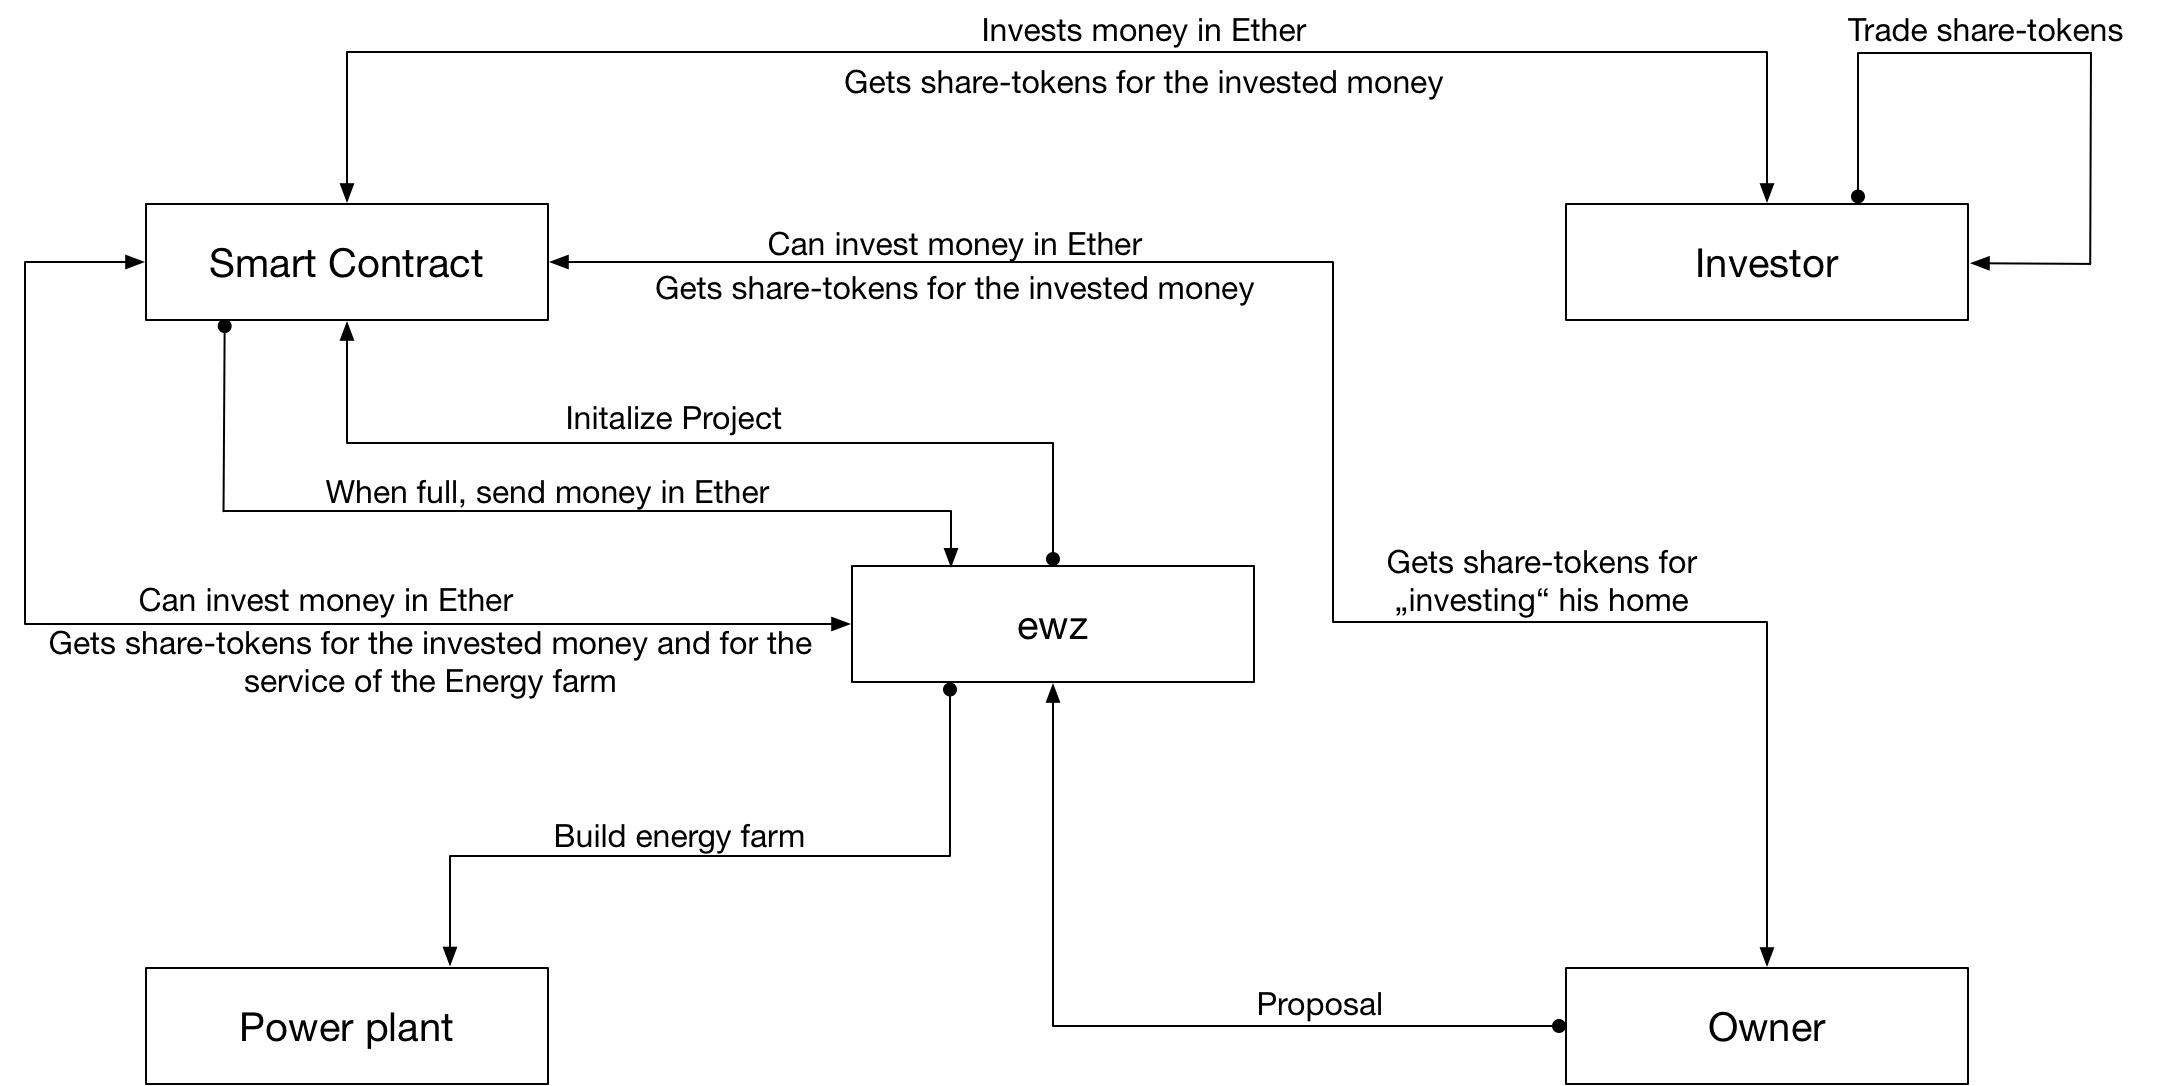
\includegraphics[width=0.8\textwidth]{images/IMG_0232.JPG}
\caption{\label{fig:blockchain}Project setup.}
\end{figure}

\subsection{Up \& Running}
Once the power plant is in operation the smart meter records the amount of power injected into the local electricity network and mints Power-Tokens according to the previously specified day or night rates.
These tokens get distributed to all investors (including the owner and ewz) in proportion to their owned Share-Tokens. The investors can then exchange those Power-Tokens back to real money or to a deduction from their own electricity bill with ewz.

%ToDo: order

\begin{figure}[h]
\centering
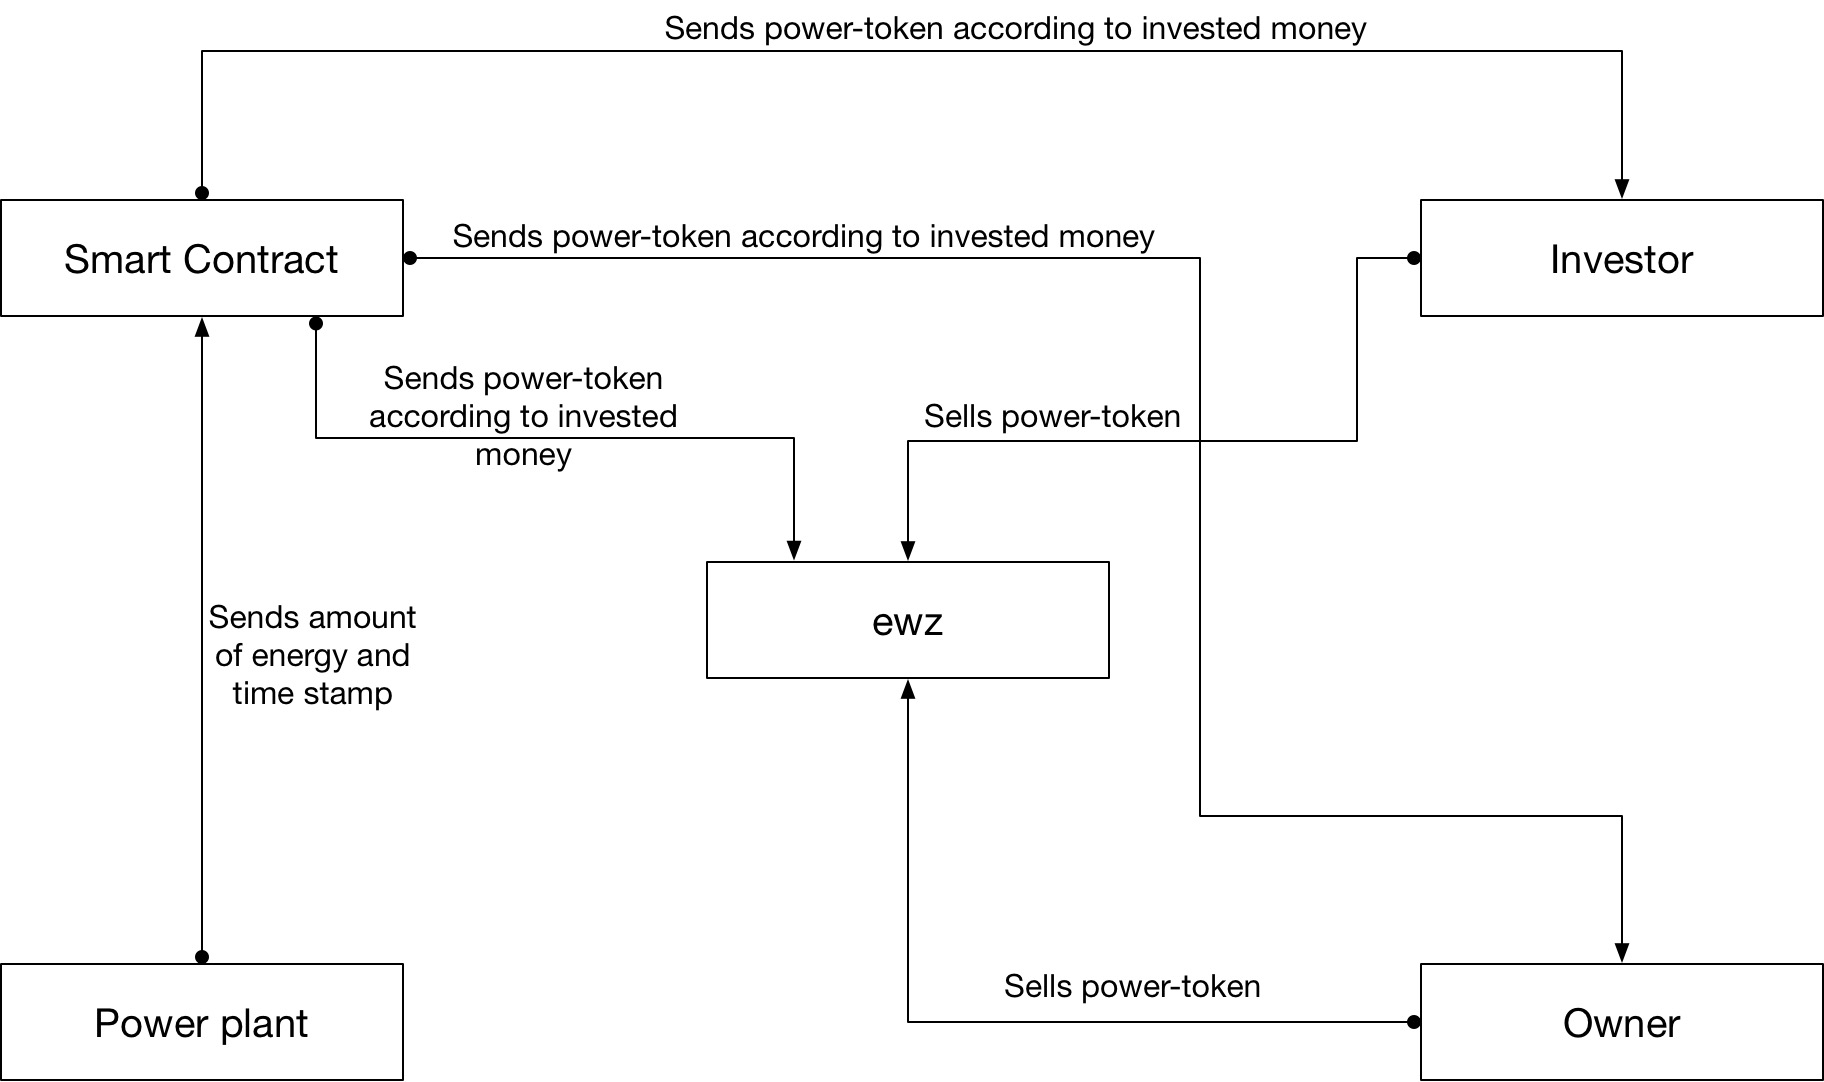
\includegraphics[width=0.8\textwidth]{images/IMG_0231.JPG}
\caption{\label{fig:Power-Token}Power-Token.}
\end{figure}
\newpage
\subsection{System Failure}
Before such a system can actually be started, there are many edge cases and system failures to consider. Of which the most important ones are discussed in this section.

The possible failures are manifold but can be roughly categorized as being of either technical or human nature. A further distinction can be made in the technical part, as being either a failure of the physical system or security breaches in the digital network. For each of these 
categories we will estimate the chance of it occurring and the severity of the damage that might be caused.

This is definitely not meant to be a conclusive analysis and because of that, it has to be regarded critically. If such a system were to be implemented, there would be many technical problems and legal issues one has to resolve, maybe using blockchain as part of the solution. A good example would be insurance and how to handle its claims. In our current version, if the project fails to acquire enough investments during the funding phase, the power plant gets irreversibly damaged or any other unsolvable problems occur which would necessitate the termination of the project, the investors in either case automatically get their invested money back.

\begin{figure}[h]
\centering
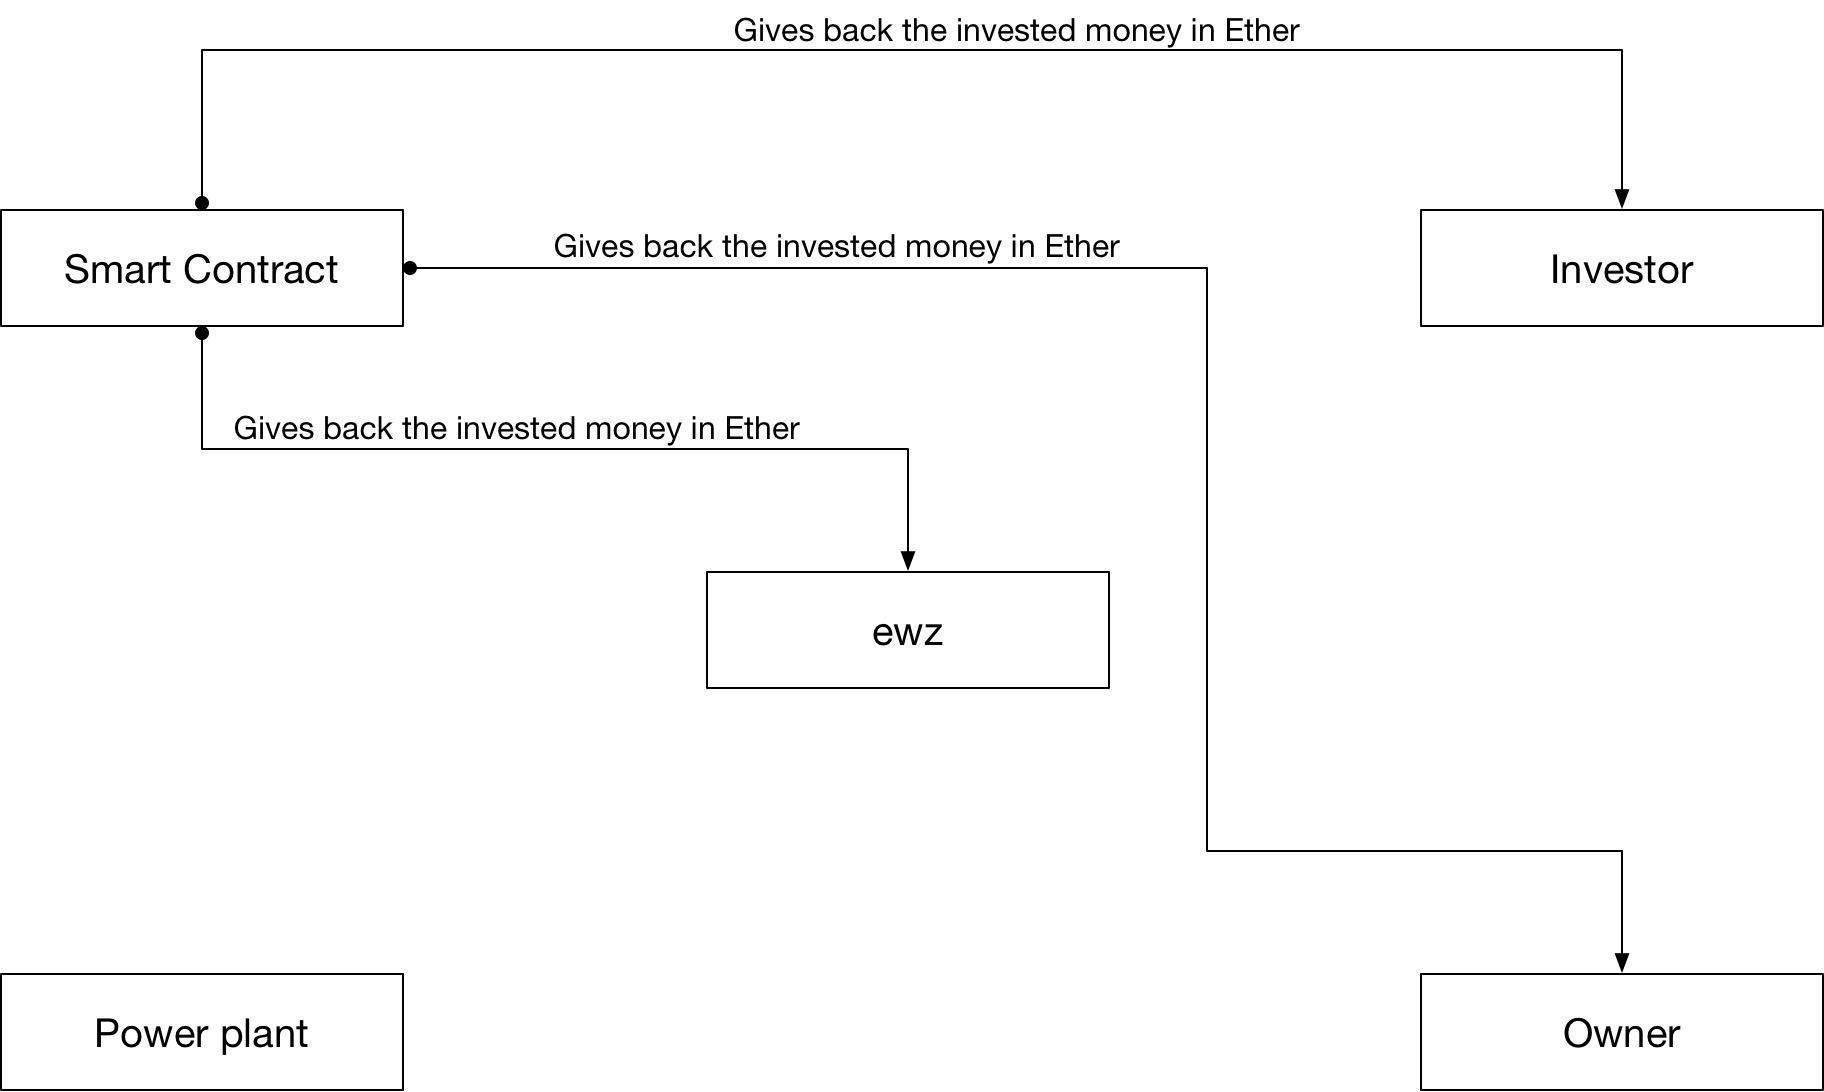
\includegraphics[width=0.8\textwidth]{images/IMG_0230.JPG}
\caption{\label{fig:terminate}Termination of a Project.}
\end{figure}

\subsubsection{Human nature}be
In this case, the owner of the system or someone else makes some sort of mistakes by trying to modify a part of the fully operational power plant. As consequence, the plant will naturally produce a reduced amount of Power-Tokens or in extreme cases none at all. This would cause no major problems for ewz since the system just doesn't feed in any electric power, but the other part namely the Power-Tokens system is still running. The real issue is, that ewz has to fix the problem of the power plant, which as one might expect requires time and money. These costs would have to either be covered by the insurance on the power plant or otherwise by the culprits.

\subsubsection{Physical nature}
Since renewable energy very often depends on the local weather conditions, there will inherently be a lot of fluctuation in the amount of power produced and in consequence in the number of Power-Tokens distributed. In the event of extreme conditions, which would lead to a prolonged interruption, the power plant could be insured to tide over the drop in earnings.

\subsubsection{Security Breaches}
Another significant problem which would have to be considered is the possibility of security breaches. In today's world of digitalization, everything is connected and anybody can try to gain access to things they should never be able to. For example, one single attacker could manage to give himself an unlimited amount of Power-Tokens (by exploiting a simple buffer overflow for instance) which would result in them losing their market value and therefore be useless to all investors. To mitigate this risk one could conduct penetration tests and code reviews, however completely ruling out any vulnerabilities is a near-impossible challenge any project of this nature has to face.

\section{Problems \& Possibilities}
\subsection{Challenge}
The goal of the challenge was to create a way for ewz to more easily expand in regions outside of their monopolistic territory. Furthermore, we were thinking about the energy market itself and all the problems it entails for its customers. We strongly believe that one of the biggest problems of renewable energy is the difficulty in joining this market and large financial investments and risks one must bear to be able to set up a power plant for renewable energy. Many people simply don't have the means to build a solar panel on their roof or put a heat pump in their basement. Therefore we set our goal to create a working proof-of-concept to improve the investment process and document our code, findings, thoughts and research along the way.

\subsection{The general idea}
To find a reliable way to incentivize people to invest in energy projects turned out to be a very difficult task. Usually us humans want to get something of value in return for investing. The solution we worked out was to create a reward or discount program coupled with the investment. This lead to the creation of a crowdfunding platform incorporating a shareholder system rewarding investments with dividend payouts based on the amount of energy produced by the power plant.

\subsection{Advantages}
One of the biggest advantages of this system is, that it leads to different ways of getting rewarded, many of which can be taken advantage of at the same time. This allows investors to more easily see the benefits of investing and assures them in the safety of their investment.

First and foremost one can invest a small amount and get money out of it in the long run by collecting dividend payments. This works similarly to the already established and well-known business entities in today's world. In our example, one receives share-tokens representing the ownership of their part of the project. Upon power generation, the dividends are paid in form of Power-Tokens. Of course, it is possible to trade those share-tokens and this way it's possible to get the full investment back.

Additionally, one can suggest a new project and provide the necessary location. This way one can build their own power plant and generate revenue by producing renewable energy. This can all be done without investing any money and by just providing the place and willingness to build a power plant. If for example one wants to put some solar panels on their roof but they lack the financial means of making this dream a reality, they can hereby gather enough funds through investors to be able to achieve those goals. Even though the house owners didn't invest any money they will still receive some of the share-tokens corresponding to the value the location has. By just investing some space and time, it is, therefore, possible to earn money.

Last but not least ewz gains access to new territory by supporting people with their projects. This way they gain influence even in other up until now monopolistic regions. After investing and building so many small projects, analyzing and advising on their technical and financial feasibility, the influence they have with customers all over the now massively increased territory will grow exponentially. Additionally, by setting up and maintaining the whole system they ensure that ewz stays irreplaceable because they are the only ones who have full access to the smart contracts. Such full access is required to add new projects, set rates and make adjustments to the power-token bank. Unfortunately in our proof-of-concept, there is currently no automated way of interacting with other energy suppliers, however, such a system could be implemented based on the Power-Token in a very similar way to how the investors get compensation.

Using the blockchain and smart contracts massively simplify the administrative tasks and reduces thereby personal expenses. Nowadays legal requirements, reviews and especially data entry consume a substantial part of a project's budget and this is exactly the point where blockchain creates massive benefits. The distribution of Power-Tokens would usually mean a periodically reoccurring manual expense, using blockchain this can all be automated. Additionally, the blockchain provides a high amount of transparency and security because the transactions are publicly visible and cannot be forged realistically.

\subsection{Disadvantages}
A major disadvantage of our current proof-of-concept is that the only currency accepted for investing is Ethereum. This means that every single investor has to use a 3rd party exchange platform to buy Ethereum first, unfortunately, some exchanges have large fees while others should not be trusted with large amounts of money. However, this problem can easily be solved by implementing a way to accept credit cards, which would, in turn, lower the technical difficulties of investing.

Unfortunately, this all sounds easier than it is, there is still much work left to be done by ewz to run a project. The whole consulting process for each and every project is done completely manually and can not reasonably be implemented on the blockchain. And after evaluating them all and finding the possible projects, they still have to be deployed on the blockchain. And this still doesn't guarantee that there's even enough interest in the project for it to reach its funding goal. The unsuccessfully collected funds can and will be refunded, however, the fees incurred in the consultation process cannot and will have to be paid by ewz.

Having all your data accessible on the Internet for everyone to see and use might not be the best thing for certain scenarios. To avoid this one could use private blockchains, however, this could lead to massive security vulnerabilities leaving the system in a useless state because customers lost their trust in it.

\subsection{The potential of blockchain}
So where can a blockchain based solution really make an impact where traditional technologies can't? One of the major advantages of a blockchain is that it's possible to automate big parts of the project, have complete traceability and ensure data integrity all at the same time. Because those things are backed up by the fundamental design of the blockchain it is possible to take advantage of those defining features in a simple way, without having to completely reinvent the wheel yourself.

\subsection{Ecological Impact}
On first sight, this all just looks like a new system to make money in a different fashion. However, this is not the only benefit because by providing a safe and easy way to invest, it would empower people from different backgrounds and with different financial means to participate and to make an impact in completely changing the use and production of energy in our society. This system strongly incentivizes people to take part in the advancement of renewable energy, which might lead to a more ecological and responsible society, further extending the lifetime of our planet and its nature.



\section{Implementation details}
\subsection{Frontend}
We implemented a web interface since the implementation on the blockchain is not very accessible for an end user without extensive knowledge of this field.
The login is implemented with the MetaMask browser plugin. In case a user opens the site without having this plugin installed, a pop up opens which informs them about the need for a plugin and automatically redirects them to the download page. The site recognizes also, whether a user is logged in and shows the login status in the upper right corner.
The website consists of three main pages, which allow the user to interact with the project structure on the blockchain. On the first Page "Projects" there is an overview of all projects which are included on the blockchain. Aside from the project name, there are important key data, for example, the monetary value of the project and the progress of its funding. Every project that is still in the funding phase, has a "Co-Fund" button on the right side. With a signed in MetaMask-Account and a click on the button, one reaches a pop-up, in which contributions to the project can be made. In return for the investment, the user receives share-tokens. The identification of the owner of the shares is done by the Ethereum wallet. The same is done with the mapping of the dividends, which the shareholder gets in the form of another token, the Power-Token. The token balances are visible on the page "My account". For a fast overview, the two most important values, amount of money invested and number of power-tokens, are written on the top of the page. Listed in a table underneath are the different investments with the corresponding interests in power-tokens. On the last page, the user has the option to exchange the earned power-tokens against Ether, which then can be converted back to money. 
At the moment the login is done by the Metamask extension for the browser, which can in a later version be replaced by a native login on the site with the user’s own Ethereum wallet. 
For a quick development, the site has been built up with several web frameworks. For the static part bootstrap was used since it is fast and easily editable and makes easy building responsive designs. Every active part was realized with plain javascript and jQuery, which allowed us manipulation of the side elements without having to reload the site.
The front end in the current state is no more than a draft to show the basic functionalities of the backend. This means that we left the web interface without a proper backend and solved most parts using JavaScript and plain HTML. In a further step, one could integrate a native login, as mentioned above, further functions to manage document projects and a detailed admin panel, which enables easier administration of the system.


\subsection{Backend}
On the blockchain, there is exactly one smart contract per project plus one global contract implementing the Power-Tokens. All of them would have to be set up by ewz. The following chapter explains, how they were implemented.

\subsubsection{Project contracts}
When ewz approves a project, they generate a smart contract for it, in which they specify the required money to finance it, the owner of the site as well as the prices for the electricity. These values are stored in the variables "CHFtoCollect", "owner", "dayprice" and "nightprice" respectively. Additionally, they add the address of the smart contract to the list of projects in the token bank (see function "addProject" below). This way only verified projects have the ability to mint Power-Tokens. The smart contract is now in the funding stage (internally this is state 1) during which other users can invest money by calling the function "buyTokens":

\begin{lstlisting}[language=Solidity, firstnumber=67]
function buyTokens() public payable{
    require(state==1);
    addHolder(msg.sender);
    if (this.balance >= CHFtoCollect * CHFtoWei){
        balanceOf[msg.sender]+=msg.value-(this.balance - (CHFtoCollect * CHFtoWei));
        msg.sender.transfer(this.balance - (CHFtoCollect * CHFtoWei)); //send too much money back.
        finalizeICO(); // finalize ICO, send coins to admin.
        missing=0;
        return;
    }
    missing -= msg.value;
    balanceOf[msg.sender]+=msg.value;
}
\end{lstlisting}

The function "addHolder" on line 69 is necessary to add the user to the list of investors. The variable "missing" stores the amount of money which still has to be collected and therefore this variable needs to be updated regularly. The difference will then be credited to the user as Share-Tokens, which are stored in the mapping "balanceOf". In the case that the sent amount is larger than what is still needed, the smart contract automatically sends back the surplus to the user and ends the funding stage, putting the project in the building stage (internally state 2), while also sending the collected money to the admin in order for him to then actually build it. The projects only leave this stage once the admin (here ewz) adds a smart meter, signaling that the project is now running, with the function "setMeter":
\begin{lstlisting}[language=Solidity, firstnumber=138]
function setMeter(address met) public{
    require(state==2 || state==3);
    require(msg.sender==admin);
    state=3;
    meter=met;
}
\end{lstlisting}

For the eventuality that the smart meter has to be replaced, we added an option to change its public address later. As soon as the first meter is set, the project enters the service stage (internally state 3). In this stage, users can no longer invest new money, but they can still transfer their shares to other users (which is actually possible in all stages). For this purpose, they have to call the function "transfer", which itself calls "transfer int": 

\begin{lstlisting}[language=Solidity, firstnumber=53]
function transfer_int(address from, address to, uint256 amount) private{
    if(from==owner || from==admin){
        require(balanceOf[from]-bonus>=amount); //lock bonus. Bonus can not be sold.
    }
    require(balanceOf[from]>=amount);
    addHolder(to);
    balanceOf[from] -= amount;
    balanceOf[to] += amount;
}
    
function transfer(address to, uint256 amount) public{
    transfer_int(msg.sender, to, amount);
}
\end{lstlisting}

At this point we should mention, that the admin and the owner receive a set share of tokens for maintenance and the provision of the building site. These additional tokens should not be tradable, which makes the if-statement on line 54 necessary. Additionally, since a smart meter has been added, it can now call the function "generateDividend":

\begin{lstlisting}[language=Solidity, firstnumber=101]
function generateDividend(uint256 energy_In_mWh, uint128 timeStamp) public{
    require(msg.sender==meter);
    require(state==3);
    require(timeStamp + 10000 > block.timestamp && timeStamp - 10000 < block.timestamp);
    require(energy_In_mWh <= maxPower);
    uint256 numPowerTokens; 
    if (dayTime){
        numPowerTokens = energy_In_mWh*dayprice;
    } else {
        numPowerTokens = energy_In_mWh*nightprice;
    }
    for(uint256 i = 0; i < index; i ++){
        PTBank.call(bytes4(keccak256("distribute(address,uint256)")), shareholders[i],(8 * numPowerTokens * balanceOf[shareholders[i]])/((CHFtoCollect * CHFtoWei * 10 )));
    }
}
\end{lstlisting}

The smart meter sends the amount of energy produced and at what time. The smart contract then calculates how many Power-Tokens each investor gets and then sends a request to the Power-Token smart contract to credit the newly added tokens to the investors. The boolean variable "dayTime" is used to determine whether the price for daytime or nighttime should be used. Which in the current version is just set by the admin with the function "setTariff". In a later implementation, this might be replaced with an automatic update by an oracle, which sets the current time and allows us thereby to determine by ourselves, whether it currently is day or night.
In the event, that the project has to be abandoned, there are multiple functions for the different stages to redistribute the money to the investors. If the project needs to be terminated in the funding stage, the admin simply calls the function "cancelICO":

\begin{lstlisting}[language=Solidity, firstnumber=87]
function cancelICO() public{
    require(state==1);
    require(msg.sender==admin);
    state=4;
    balance = this.balance;
    distributeETH();
}

\end{lstlisting}
Which checks the needed requirements and then calls "distributeETH":


\begin{lstlisting}[language=Solidity, firstnumber=129]
function distributeETH() private{
    balanceOf[owner]-= bonus; //destroy bonus
    balanceOf[admin]-= bonus; //destroy bonus
    
    for(uint256 i = 0; i < index; i ++){
        shareholders[i].transfer((balance * balanceOf[shareholders[i]])/((CHFtoCollect * CHFtoWei)-missing));
    }
}
\end{lstlisting}

This function simply returns to each shareholder the amount of ether in accordance with their shares. Here one again has to take in consideration the additional shares of the admin and the owner, which have to be deducted since they do not correspond to actual money invested. This works similarly in the event that the project is already in one of the later stages, for example, if the power plant gets destroyed and the insurance pays the money invested to the ewz. In this case, the admin has to call "terminateProject":

\begin{lstlisting}[language=Solidity, firstnumber=120]
function terminateProject() public payable{
    require(state==2 || state == 3);
    require(msg.sender==admin);
    require(msg.value >= (CHFtoCollect * CHFtoWei));
    state=4;
    balance = this.balance;
    distributeETH();
}
\end{lstlisting}

Although this only works if the call also contains enough money. Which will then again trigger a call of "distributeETH". Should there ever be a need to terminate a project without the necessary funds, then the admin can offer the investors off-chain to buy their shares for a lower price.

\subsubsection{Power-Token}
In the smart contract "PowerToken" are the Power-Tokens handled. For this purpose a few important variables are required:

\begin{lstlisting}[language=Solidity, firstnumber=4]
mapping (address => uint256) public balanceOf;
mapping (address => uint8) public projects;
\end{lstlisting}

In the mapping "balanceOf" each investors balance of Power-Token is stored. The mapping "projects" is used to store which addresses on the blockchain are actual projects and therefore allowed to generate Power-Tokens.
Once the smart contract is deployed, ewz can add projects using the function "addProject":

\begin{lstlisting}[language=Solidity, firstnumber=38]
function addProject(address pc) public{
    require(msg.sender == admin);
    projects[pc] = 1;
    projects_addr[index]=pc;
    index+=1;
}
\end{lstlisting}

Which simply changes the permissions of the project, given that the function is called by the original creator. The project can then call the function "distribute":

\begin{lstlisting}[language=Solidity, firstnumber=43]
function distribute(address to, uint256 amount) public{
    require(projects[msg.sender] == 1);
    balanceOf[to] += amount;
    generated[msg.sender] += amount;
}
\end{lstlisting}

This then simply adds the specified amount to the correct investor's balance. An investor can then transfer his Power-Tokens to someone else using the function "transfer":

\begin{lstlisting}[language=Solidity, firstnumber=32]
function transfer(address to, uint256 amount) public{
    require(balanceOf[msg.sender]>=amount);
    balanceOf[msg.sender] -= amount;
    balanceOf[to] += amount;
}
\end{lstlisting}

Provided he does have a sufficient number to do so. Alternatively, he can also exchange his Power-Tokens for etherum with the function "sellTokens":

\begin{lstlisting}[language=Solidity, firstnumber=17]
function sellTokens(uint256 amount) public{
    require(amount*buyBackRate <= this.balance);
    balanceOf[msg.sender] -= amount;
    msg.sender.transfer(amount*buyBackRate);
}
\end{lstlisting}

For this transaction an exchange rate has to be specified in the variable "buyBackRate". The value of which can be changed by the function "setRate":

\begin{lstlisting}[language=Solidity, firstnumber=22]
function setRate(uint256 rate) public {
    require(msg.sender == oraclize);
    buyBackRate = rate;
}
\end{lstlisting}

The variable "oraclize" is used to record an address, here a smart contract, who is then allowed to change the exchange rate. In practice, this is necessary in order to be able to set up a smart contract, which periodically updates the exchange rate with a current value obtained from an oracle (for example oraclize). This address can be changed by the admin through the function "setOraclize":

\begin{lstlisting}[language=Solidity, firstnumber=27]
function setOraclize(address oc) public {
    require(msg.sender == admin);
    oraclize = oc;
}
\end{lstlisting}


\section{Difficulties}
Since the concept is very scalable and could be used for a wide variety of other sectors, extending the code is inevitable to make the system fit new challenges. Because of the static nature of the blockchain technology, an update of the functionality is complicated and asociated with considerable effort. A concrete example is a change in the distribution mechanism of the power-token. Since every project contract references to this contract, it would mean that it must be changed everywhere. A solution to this problem would be an external reference, per example a database with the corresponding references to the contracts, but such a solution defeats the decentralization of information and independence of the system, one of the major advantages of the blockchain technology.
Data management with blockchain turned out to be way more complex than with traditional databases. While normal databases, once requested, deliver data simultaneously or somewhat ordered, a request to the blockchain is more complex and much more difficult to fetch correctly. The fragmentation of the data at different locations in the blockchain and the asynchronous nature of the requests via web3.js made retrieving bigger sets of data very laborious.
Since blockchain is a relatively new field, there are only a few comprehensive sources to rely on while developing applications. Fortunately, plenty of experts attended the event and also helped us implement our ideas on the blockchain.


\section{Conclusion}
The last two days were a rush. We did a lot, but there were still plenty ideas which we couldn’t integrate into the final version. 
In the end, we had a rough sketch of a blockchain based platform, which provides the possibility of handling an unsupervised crowdfunding application for investing in energy plant projects, which automatically distributes the dividends to the different investors. This functionality seems to be working perfectly and the technology blockchain is in our eyes a perfect solution for such an application. 
Although the core is working, there are plenty things that still have to be done before the application could be called finished. This means, for example, more steps in building a power plant should be automated. With our system ewz has still a lot of work to do until a project is up and running. Also to expand ewz territory the system needs an entire additional part to automate this process and ensure that it doesn't produce a large amount of office work for ewz. These are just some examples what has to be done to make a reliable, attractive solution for all involved parties. 
Our approach is based on a rather simplified project structure with a lot of responsibility on the side of the initial funder and on top of that it doesn’t implement solutions on how to handle bigger revisions of a plant. This means that the investors must get some kind of insurance that the initial funder will set up the plant as promised and will not overdraw the set project budget. There must be also a verification system for investors and project starters to minimize the chance of being scammed. The documentation of running costs would have to be improved so that every investor can look up how much money is used for maintenance of the plant. 
Aside from the business model, there are also some technical points that have to be tackled. Even though the blockchain technology is extremely difficult to tamper with, there’s still a risk that smart contacts get exploited. This could be prevented by having a security audit done by a specialized company. 

\subsection{Future, expandability}
The concept of crowdfunded projects with a systematic distribution of interest is applicable on many other topics than just on small power plants. Especially because the focus doesn’t lie mainly on trust and surveillance in this application. The automated process of emitting interest, having a system of shares, which allow easy, non-regulated, but safe transfer and resilience against outage of single parts of the system is what makes the system interesting. Through the high grade of automation, a big part of the administrative tasks can be designed more efficiently or can be replaced completely by the blockchain. For this reason, it is also possible to integrate this topic in environments where the output/interest cannot be as safely measured as in our business case. Especially with the rise of a shared economy, there will be a spot for blockchain applications like this one in the future. Services like sharely.ch could build up something like our application to track the lending of tools and devices to other people and track a lending score for each user, which enables the user to borrow stuff from other people with his score points.

To make our system interesting to the public there is as mentioned above a lot of work to do on a technological basis but also on the publicity side. The system is not working if not enough people participate. But it is a good way to get started.
%
% Example citation \cite{einstein}
%
%\begin{lstlisting}[language=Solidity]
%
%\end{lstlisting}
%
\clearpage

%----------------------------------------------------------------------------------------
%	ATTACHMENT SECTION
%----------------------------------------------------------------------------------------

%\pagenumbering{roman}
%\setcounter{page}{1}
%\section*{Attachments}
%\clearpage

%----------------------------------------------------------------------------------------
%	BIBLIOGRAPHY SECTION
%----------------------------------------------------------------------------------------
%\bibliographystyle{unsrt}
%\bibliography{bibliography}

\end{document}